\documentclass[11pt]{article}
\usepackage{amsmath}
\usepackage{amssymb}
\usepackage{float}
\usepackage[T1]{fontenc}
\usepackage{graphicx}
\usepackage[utf8]{inputenc}
\usepackage{mathtools}
\usepackage{txfonts}
\usepackage{wasysym}
\usepackage[svgnames]{xcolor}
\usepackage[paperheight=29.7cm,paperwidth=21.0cm,left=2.54cm,right=2.54cm,top=2.54cm,bottom=2.54cm]{geometry}
\usepackage[hidelinks]{hyperref}
\usepackage{xurl}

\setlength\parindent{0pt}
\renewcommand{\arraystretch}{1.3}
\begin{document}
Headings: $-$

\begin{itemize}
	\item Abstract

	\item Keywords

	\item Introduction

	\item A review of literature / Previous Works on Respiratory Voice Diagnostics

	\item Methodology

	\item Features Info

	\item Models

	\item Results and Discussion

\vspace{37\baselineskip}
\end{itemize}
{\LARGE \textcolor[HTML]{0E101A}{Abstract: }}

\textcolor[HTML]{0E101A}{ }

\textcolor[HTML]{0E101A}{COVID$-$19} was declared a global pandemic on 11 March 2020; since then much technological advancement is already in place to identify COVID$-$19 patients. We present a COVID$-$19 cough classifier that would help in contactless detection of COVID$-$19 patients by analysing their audio cough samples. The report demonstrates five machine learning classification models and combines those models into an ensemble model with 26 dominant features. The proposed method has been examined on both COVID$-$19 positive and healthy individuals' cough recordings. The results are promising, scoring accuracy of 99.3$\%$, a sensitivity of 99$\%$ on validation data with an Area under the ROC curve of 0.97, all while maintaining interpretability.\textcolor[HTML]{0E101A}{}

\textcolor[HTML]{0E101A}{ }

\vspace{1\baselineskip}
{\LARGE \textcolor[HTML]{0E101A}{Introduction:}}

\textcolor[HTML]{0E101A}{ }

\textcolor[HTML]{0E101A}{On 11 March 2020, World Health Organization (WHO) declared COVID$-$19 a global pandemic. COVID$-$19 is caused by SARS$-$CoV$-$2(Severe Acute Respiratory Syndrome Corona$-$Virus). It starts by infecting the mucous membranes within the throat and moves down the respiratory tract leading to the lungs, with coughing being a common symptom [1]. Cough sound contains underutilised pulmonary health information which can be used for analysis. Until 16 June 2021, more than 177 million cases confirmed COVID$-$19 infections in more than 200 countries. Based on World Health Organization (WHO) statistics, close to 3.8 million people passed away after getting infected by the virus [2]. As we eagerly await new drug and vaccine discoveries, a highly effective method to regulate the deadly virus spread is frequent testing at scale to reduce transmission [3]. This has led to a dire necessity for screening and diagnostic solutions that can be implemented globally.}

\textcolor[HTML]{0E101A}{ }

\textcolor[HTML]{0E101A}{Methods like X$-$rays and Chest CT scans have been used to differentiate between COVID$-$19 and non COVID$-$19 patients [4]. Furthermore, these methods suggest that COVID$-$19 affects the respiratory system in a distinctive way [5]. Therefore, vital information about the respiratory system and the pathologies involved are carried in the cough sounds [6].            }

\textcolor[HTML]{0E101A}{ }

\textcolor[HTML]{0E101A}{AI has many applications in speech and audio analysis, which can be implemented in the screening and early discovery of the infected people process, which could help curb and decrease the number of infected people. A cough audio modelling can provide diagnostic leads by implementing various machine learning tools and algorithms with advanced feature extraction techniques and robust classification models. Given the requirement of identifying COVID$-$19 patients, Machine Learning algorithms are extensively used to distinguish between COVID$-$19 and non COVID$-$19 patients by analysing the cough patterns. This paper identifies the various characteristics/pattern of COVID$-$19 cough by performing specific feature extraction techniques.}

\textcolor[HTML]{0E101A}{ }

\textcolor[HTML]{0E101A}{Implementing a classification algorithm and capable hardware can process cough audio to decrease the strain on the chemical labs and avoid chemical and toxic waste. Results can be displayed almost immediately with the help of machine learning classification algorithms. This paper presents cough audio processing from patients and analyses the waveforms based on different parameters to classify the audio into a COVID$-$19 patient or a healthy person. In the classification part, we use the five most interpretable machine learning classification algorithms and provide the 25 dominant features to these five classifiers to obtain the result and make an ensemble model that would be the most appropriate classifier for realistic implementation of COVID$-$19 cough detection.}

\textcolor[HTML]{0E101A}{ }

{\LARGE \textcolor[HTML]{0E101A}{A Review of literature:}}

\textcolor[HTML]{0E101A}{ }

\textcolor[HTML]{0E101A}{This review attempts to summarise the vital studies in cough detection and identify diseases based on cough audio samples' features like frequency, duration, and intensity. A review of the literature is provided hereunder, keeping in view the current technological advancements specific to the focus of this research. In recent years, numerous studies have suggested acoustic features to identify respiratory diseases in cough signals. Furthermore, conditions associated with the respiratory system can be detected using machine learning algorithms analysis. Machine learning algorithms can also process respiratory data and coughs to diagnose COVID$-$19 [8][11]. }

\textcolor[HTML]{0E101A}{ }

\textcolor[HTML]{0E101A}{Abeyratne et al. [9] examined the differences in pneumonia, asthma and bronchitis coughs. This paper extracted features from the cough sound such as Mel Frequency Cepstrum Coefficients, Zero Crossing, Formant frequencies and non$-$Gaussianity score; performed feature selection based on the p$-$value of the features. The Logistic Regression Model trained on recordings from 91 subjects showed a sensitivity of 80$\%$ and specificity of 73$\%$ on the Validation set. They also provided evidence supporting the hypothesis that cough carries information on the state of the lower respiratory tract.  }

\textcolor[HTML]{0E101A}{ }

\textcolor[HTML]{0E101A}{In the system proposed by Belkacem et al. [10], the cough recording is initially passed through a cough detection system, a source separation system and then features such as Shannon Entropy (SH), Zero Crossing Rate and Mel$-$Frequency Cepstral Coefficients are extracted from the recording which is then passed through Deep Neural Network (DNN). A logarithmic scaled Mel$-$spectrogram has also been used for feature extraction, passed through a fully convolutional network (FCN). The authors also designed a pipeline in MATLAB to analyse the cough recordings, which consists of computing Fast Fourier Transform (FFT), Signal energy to extracting the features aforementioned.}

\textcolor[HTML]{0E101A}{ }

\textcolor[HTML]{0E101A}{Chatrzarrin et al. [12] have listed pre$-$processing and feature extraction techniques obtained from cough signals to classify them into dry and wet coughs. In a study carried out by Vikrant Et al. [13], the cough sound signals of the patients were classified into different respiratory ailments using a Support Vector Machine (SVM) classifier with the extraction of 3 features. SVM classifier yields an accuracy of 98.9$\%$ with True Positive Rate (TPR) ranging from 94$\%$ to 100$\%$. In another study carried out by Matos Et al. [14], the hidden Markov models (HMMs) have been used to detect cough sounds with the extraction of features like linear predictive coding (LPC) coefficients and Mel frequency cepstral coefficients (MFCC). The algorithm used in the paper was able to identify 82$\%$ of the events of coughing correctly. }

\textcolor[HTML]{0E101A}{ }

\textcolor[HTML]{0E101A}{Imran et al. have made an app to classify COVID$-$19 cough from an audio recording with precision close to 90$\%$ [16]. They used a model pre$-$trained on general sounds and then tuned on COVID$-$19 data. Their app uses a mediator to combine the prediction of a Deep Learning model that uses a mel$-$spectrogram, consists of a Convolutional Neural Network (CNN) and a Machine Learning model which uses Mel Frequency Cepstrum coefficients (MFCC) as features to generate predictions.}

\textcolor[HTML]{0E101A}{ }

\textcolor[HTML]{0E101A}{Sharma et al. have created a database consisting of respiratory sounds like coughing, breathing, and voice known as Coswara for COVID$-$19 detection [17]. The Random Forest (RF) model trained on Coswara data gave a mean accuracy of 70$\%$ for coughing. In the paper by Wang et al. [18], Voice Activity Detection (VAD) has been done based on the similarity of Cepstral Coefficients. The usage of MFCC has proven to be the most suitable method for VAD in a noisy background compared to other features.}

\vspace{1\baselineskip}
{\LARGE Methodology:}

\vspace{1\baselineskip}
Accuracy $=$ 98.55$\%$ $\pm$ 0.6$\%$

Dataset consisting of 1443 cough audio recordings out of which 111 were that of COVID$-$19 positive patients and 1340 were that of healthy individuals was obtained out of which 164 recordings are from University of Manchester [19] and the rest 1279 recordings are taken from Indian Institute of Science, Bangalore [17]. As the dataset was imbalanced, SMOTE Data balancing technique was used. This technique has proven to be successful in the field of cough detection and classification [20]. 

\vspace{1\baselineskip}
Our speech signals consist of a set of information. The determination and capturing of such features would help us distinguish between a variety of coughs. For extracting these features, the cough recordings are in \textit{.wav} format, and these waves are digitalised. These are converted into a one$-$dimensional array of digital values using sampling technique. These digital values represent the amplitude, frequency at that given instance. Here the sampling rate is fixed to 22050 for all the recordings. A total of 26 features were extracted from each cough recording, such as MFCC (first 20 coefficients), Chroma STFT, Root Mean Square Energy, Spectral Centroid, Spectral Roll off and Zero Crossing Rate.

\vspace{1\baselineskip}
{\Large \textbf{Feature Extraction}{\large \textbf{:}}}

\vspace{1\baselineskip}
\begin{itemize}
	\item {\large \textit{Zero Crossing Rate}}

The Zero Crossing Rate (ZCR) [15] is the number of times the signal changes sign within a frame.

\vspace{1\baselineskip}
\begin{equation}
ZCR =\frac{1}{T - 1}\sum_{t = 1}^{T - 1} \lambda\left(s_{t}s_{t - 1}<0\right)
\end{equation}


{\large \ \ \ \ }

Where \( \lambda\) $=$ 1 when the sign of \( s_{t}\) and \( s_{t - 1}\) differ and \( \lambda\) $=$ 0 when the sign of \( s_{t}\) and \( s_{t - 1}\) are same.

\vspace{1\baselineskip}
	\item {\large \textit{Chroma STFT}}

A 12$-$element representation of spectral energy where the bins represent the 12 distinctive pitch classes used to study music (semitone spacing) where each representation indicates how much energy each pitch class has. The figure below uses short term Fourier transformation in order to compute Chroma features.  These features carry harmonic and melodic characteristics of the audio while being robust to changes in timbre.

\vspace{1\baselineskip}
\begin{figure}[H]
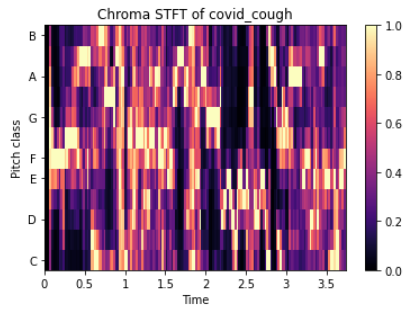
\includegraphics[width=7.34cm,height=5.47cm]{./images/image1.png}
\end{figure}


	\item \textit{MFCC}

Mel frequency cepstral coefficients is a compact representation of the spectrum, a primary feature in research areas that includes audio signals ranging from detecting cough sounds to automatic speech recognition [21].

\vspace{1\baselineskip}
MFCC represents the sound spectrum by converting the audio signal via a sequence of steps to imitate the vocal tract. MFCC can completely capture the characteristics of the spectrum and simulate the human's auditory function, whose approximation of speech is linearly spaced on the frequency scale. In filter$-$source theory, "the source is the vocal cords, and the filter represents the vocal tract."

\vspace{1\baselineskip}
Characteristics like shape and length of the vocal tract determine how sound is outputted from an individual, and the \textit{Cepstrum coefficients} describe the filter, i.e., represent sound in a structured manner [22]

\begin{figure}[H]
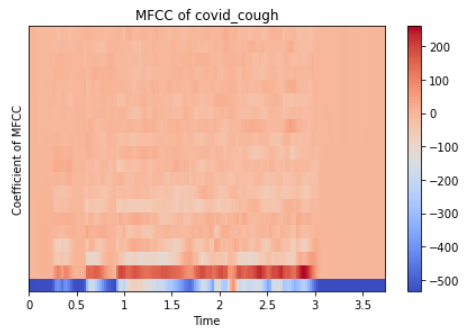
\includegraphics[width=7.4cm,height=5.31cm]{./images/image2.png}
\end{figure}


	\item \textit{Root Mean Square Energy}

The energy of a signal is give by its total magnitude. For audio signals, this characterises to how loud the signal is. RMSE is the square root of the mean square (the average of the squares of the magnitude of the audio frames).[23]

\vspace{1\baselineskip}
\begin{equation}
\sqrt{\frac{1}{N}\sum_{n}^{} \vert x(n)\vert^{2}}
\end{equation}


\vspace{1\baselineskip}
	\item \textit{Spectral Roll off}

Spectral Roll$-$off is the frequency below which lies a specified percentage of the total spectral energy \( N\) lies.

\vspace{1\baselineskip}
\begin{equation}
\text{Roll}\text{ - }\text{off}\text{ } = \sum_{k = b_{1}}^{d} s_{k} = N\left(\sum_{k = b_{1}}^{b_{2}} s_{k}\right)
\end{equation}


\vspace{1\baselineskip}
where \( s_{k}\) is the spectral value at bin \( k\), \( N\) is the percentile cutoff, and \( b_{1}\) and \( b_{2}\) are the band edges.

\vspace{1\baselineskip}
	\item \textit{Spectral Centroid}

Spectral centroid is a measure to compute the "centre of mass" of a given spectrum. It tells us about sound "brightness", which indicates the amount of high$-$frequency content in a sound. This is like a weighted mean:

\vspace{1\baselineskip}
\begin{equation}
f_{c} =\frac{\sum_{k}^{} S(k)f(k)}{\sum_{k}^{} S(k)}
\end{equation}


\vspace{1\baselineskip}
where \( S(k)\) is the spectral magnitude at frequency bin \( k\), \( f(k)\) is the frequency at bin \( k\).

\vspace{1\baselineskip}
	\item \textit{Spectral Bandwidth}

The spectral bandwidth is defined as the extent of the power transfer function around the centre frequency [24]. 

\vspace{1\baselineskip}
\begin{equation}
\left(\sum_{k}^{} S(k)\left(f(k) - f_{c}\right)^{p}\right)^{\frac{1}{p}}
\end{equation}


\vspace{1\baselineskip}
where \( S(k)\) is the spectral magnitude at frequency bin \( k\), \( f(k)\) is the frequency at bin \( k\), and \( f_{c}\) is the spectral centroid.

\vspace{3\baselineskip}
{\Large \textbf{Classifier Architectures:}}

\vspace{1\baselineskip}
Five different classification models have been trained and tested on the dataset, keeping in mind the interpretability and explainability of the models:

\vspace{1\baselineskip}
$\ast$The idea here is to combine models with more explainability and more precision$\ast$

\vspace{1\baselineskip}
	\item \textit{Logistic Regression}

We start with Logistic Regression. Logistic Regression has been found to be superior to other models such as Decision Trees, SVM, ANN in the field of Clinical Diagnosis [25]. The output of a logistic regression model is given below:

\vspace{1\baselineskip}
\begin{equation}
P =\frac{1}{1 + e^{ - (a + b\mathbf{x})}}
\end{equation}


\vspace{1\baselineskip}
where \( a\) and \( b\) are the model parameters. \( P\) is interpreted as probability and hence is used for binary classification. Hyperparameter tuning and Regularisation has been done on the Logistic Regression model to reduce overfitting. Three types of penalties were considered used to minimise the loss function: lasso, ridge and elastic net penalty (same weights of l1 and l2) and used AUC scores to compare the models. 

\vspace{1\baselineskip}
	\item \textit{Explainable Boosting Classifier}

Explainable Boosting Classifier [26] is a glass$-$box model created by Microsoft. It is a modification of a generalised additive model (GAM), also known as GA\textsuperscript{2}M model [27] and is of the form:

\vspace{1\baselineskip}
\begin{equation}
g(E[y]) = \beta_{0} + \sum f_{i}\left(x_{i}\right) + \sum f_{i,j}\left(x_{i},x_{j}\right)
\end{equation}


\vspace{1\baselineskip}
Where \( g\) is the link function that adapts the GAM to different settings such as Regression or classification,  \( f_{i}\) is a feature function that is learned by Explainable Boosting Classifier using machine learning techniques like Gradient Boosting and Bagging, \( f_{i,j}\) represents the pairwise interaction function [29] of these features. Being an additive model, contributions of each feature to the prediction can be observed and hence these contributions can be understood, making the model completely interpretable.

\vspace{1\baselineskip}
	\item \textit{Decision Tree Classifier }

Decision Tree Classifier [30] is a tree$-$structured classifier that replicates the human thinking ability while making a decision. The tree structure of the Decision Tree Classifier is ideal for capturing the interactions between the model's features, hence maintaining the interpretability of the model.  The relation between outcome \(\hat{y}\) and features \( x\) is given by [31]:

\vspace{1\baselineskip}
\begin{equation}
\hat{y} =\hat{f}(x) = \sum_{m = 1}^{M} c_{m}I\left\{ x\in R_{m}\right\} 
\end{equation}


\vspace{1\baselineskip}
Where \( I\left\{ x\in R_{m}\right\}\) is an identity function that returns 1 if \( x\) is a subset of \( R_{m}\) otherwise 0. If an instance falls into a leaf node \( R_{l}\), the predicted outcome is \(\hat{y} = c_{l}\), where \( c_{l}\) is the average of all training instances in the leaf node \( R_{l}\). The selection of best attributes (also known as Attribute selection measure) is made using the Information Gain (or Entropy) technique, and the maximum depth of the tree is taken as 5.

\vspace{1\baselineskip}
	\item \textit{Random Forest Classifier}

Random Forest Classifier [31] is a supervised learning algorithm that creates, fits decision trees on randomly selected subsamples, and selects the best solution/prediction among these trees by voting and aggregation in classification and regression. These individual trees are generated using indicators such as information gain and the Gini index. Random Forest Classifier is also a good indicator of feature importance [32]. RFC also overcomes the overfitting caused by individual decision trees through the randomness of subsample and features’ selection.

\vspace{1\baselineskip}
	\item \textit{XG Boost}

XG Boost [33] is a supervised learning algorithm that implements a process called boosting which is an ensemble learning technique which corrects for deficiencies in previous models. 

\vspace{1\baselineskip}
	\item {\Large \textit{Ensemble Model}}

\vspace{31\baselineskip}
Feature's extraction such as Short$-$Time Fourier Transform (STFT), Mel Filter$-$Bank (MFB), and MFCC have been evaluated using classifiers such as CNN and LSTM. Moreover, the differentiation among coughs has been made based upon the acoustic features [8  $-$ I. D. Miranda, A. H. DIacon and T. R. Niesler, "A Comparative Study of Features for Acoustic Cough Detection Using Deep Architectures," Proceedings of the Annual International Conference of the IEEE Engineering in Medicine and Biology Society, EMBS, pp. 2601$-$2605, 2019.]

\vspace{2\baselineskip}
\textit{Check:}

\vspace{1\baselineskip}
	\item An algorithm for matching patterns, recognising and differentiating speech is developed based on using the MFCC as the extracted features and the principle of collecting the correlation coefficients [7 $-$ A. Pramanik and R. Raha, "Automatic Speech Recognition using correlation analysis," Proceedings of the 2012 World Congress on Information and Communication Technologies, WICT 2012, pp. 670$-$ 674, 2012.]

\vspace{1\baselineskip}
	\item A study in [2 $-$ Al$-$khassaweneh M, Abdelrahman Ra’ed Bani. A signal processing approach for the diagnosis of asthma from cough sounds. J Med Eng Technol. 2013;37(3):165–71.] showed that the coughs from asthmatic patients had a measurably higher energy signature

\vspace{1\baselineskip}
	\item The acoustic sound of a cough is generated by the contractions of the respiratory muscles, cough's 3 phases [10]

\vspace{1\baselineskip}
	\item A comprehensive review of the detection and analysis of voice pathology from acoustic analysis may be found in [8 $-$ Boyanov Boyan, Hadjitodorov Stefan. Acoustic analysis of pathological voices. a voice analysis system for the screening of laryngeal diseases. IEEE Eng Med Biol Mag. 1997;16(4):74–82.]

\vspace{1\baselineskip}
	\item (See: \url{https://www.kaggle.com/himanshu007121/fork-of-covid-19-cough-classification-7b7322/edit} and \url{https://rramnauth2220.github.io/blog/posts/code/200525-feature-extraction.html} $+$ Mathpix $+$ \href{file:///C:/Kgp/CP/Preparation/COVID\%20Project/Audio\%20Files/Research\%20Papers/COVID\%20Cough\%20Papers/2012.01926.pdf}{file:///C:/Kgp/CP/Preparation/COVID$\%$20Project/Audio$\%$20Files/Research$\%$20Papers/COVID$\%$20Cough$\%$20Papers/2012.01926.pdf} $+$ \href{file:///C:/Kgp/CP/Preparation/COVID\%20Project/Audio\%20Files/Research\%20Papers/COVID\%20Cough\%20Papers/Machine\%20Learning\%20based\%20COVID-19\%20models\%20research.pdf}{file:///C:/Kgp/CP/Preparation/COVID$\%$20Project/Audio$\%$20Files/Research$\%$20Papers/COVID$\%$20Cough$\%$20Papers/Machine$\%$20Learning$\%$20based$\%$20COVID$-$19$\%$20models$\%$20research.pdf} $+$ \url{https://towardsdatascience.com/how-i-understood-what-features-to-consider-while-training-audio-files-eedfb6e9002b} $+$ \href{file:///C:/Kgp/CP/Preparation/COVID\%20Project/Audio\%20Files/Research\%20Papers/COVID\%20Cough\%20Papers/Urban\%20Sound\%20Classification\%20Using\%20Convolutional\%20Neural\%20Network\%20and\%20Long\%20Short\%20Term\%20Memory\%20Based\%20on\%20Multiple\%20Features.pdf}{file:///C:/Kgp/CP/Preparation/COVID$\%$20Project/Audio$\%$20Files/Research$\%$20Papers/COVID$\%$20Cough$\%$20Papers/Urban$\%$20Sound$\%$20Classification$\%$20Using$\%$20Convolutional$\%$20Neural$\%$20Network$\%$20and$\%$20Long$\%$20Short$\%$20Term$\%$20Memory$\%$20Based$\%$20on$\%$20Multiple$\%$20Features.pdf})

\vspace{18\baselineskip}
{\LARGE Results: COVID19 Classification Performance}

\vspace{2\baselineskip}
\begin{figure}[H]
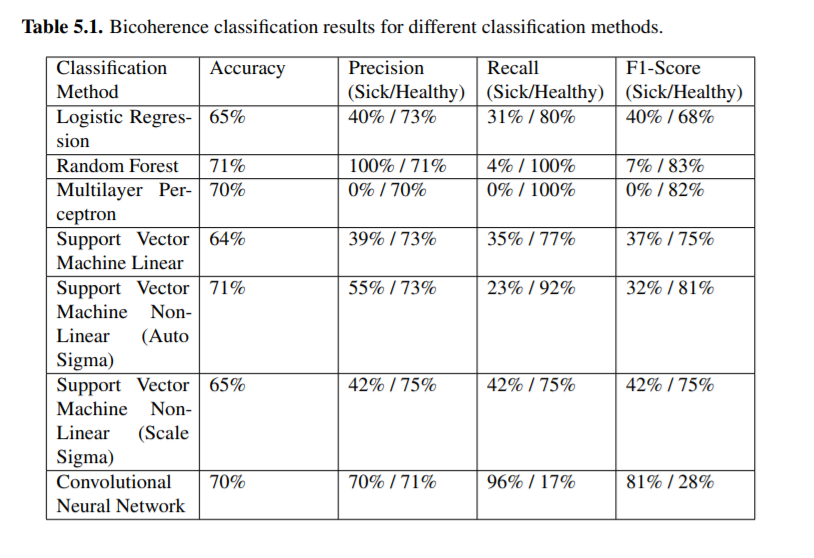
\includegraphics[width=10.4cm,height=7.13cm]{./images/image3.png}
\end{figure}


\vspace{1\baselineskip}
\begin{figure}[H]
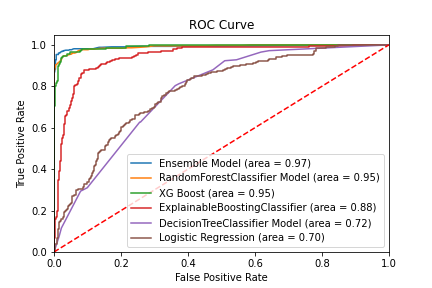
\includegraphics[width=8.02cm,height=5.35cm]{./images/image4.png}
\end{figure}


\vspace{1\baselineskip}
\begin{figure}[H]
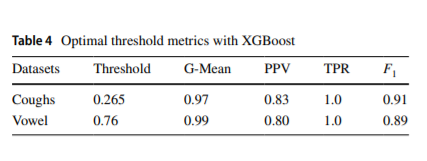
\includegraphics[width=11.29cm,height=4.26cm]{./images/image5.png}
\end{figure}


( \href{file:///C:/Kgp/CP/Preparation/COVID\%20Project/Audio\%20Files/Research\%20Papers/COVID\%20Cough\%20Papers/Mouawad2021_Article_RobustDetectionOfCOVID-19InCou.pdf}{file:///C:/Kgp/CP/Preparation/COVID$\%$20Project/Audio$\%$20Files/Research$\%$20Papers/COVID$\%$20Cough$\%$20Papers/Mouawad2021\_Article\_RobustDetectionOfCOVID$-$19InCou.pdf} )

\vspace{1\baselineskip}
Also:

	\item \href{file:///C:/Kgp/CP/Preparation/COVID\%20Project/Audio\%20Files/Research\%20Papers/COVID\%20Cough\%20Papers/Signal\%20Analysis\%20and\%20Classification\%20of\%20Audio\%20Samples\%20-\%20COVID-19.pdf}{file:///C:/Kgp/CP/Preparation/COVID$\%$20Project/Audio$\%$20Files/Research$\%$20Papers/COVID$\%$20Cough$\%$20Papers/Signal$\%$20Analysis$\%$20and$\%$20Classification$\%$20of$\%$20Audio$\%$20Samples$\%$20$-$$\%$20COVID$-$19.pdf} – See Discussion

	\item Comment on existing methods

\vspace{1\baselineskip}
{\LARGE Reference:}

\vspace{1\baselineskip}
[1] \textcolor[HTML]{333333}{Mouawad, P., Dubnov, T. $\&$ Dubnov, S. Robust Detection of COVID$-$19 in Cough Sounds. \textit{SN COMPUT. SCI.} \textbf{2, }34 (2021). \url{https://doi.org/10.1007/s42979-020-00422-6}}

\textcolor[HTML]{333333}{[2] }[Online]. Available: \url{https://www.worldometers.info/coronavirus/} [Accessed 16 June 2021].

[3] Kucharski, A. J.; Klepac, P.; Conlan, A.; Kissler, S. M.; Tang, M.; Fry, H.; Gog, J.\ \ \ \ ; and Edmunds, J. 2020. Effectiveness of isolation, testing, contact tracing and physical distancing on reducing transmission of SARS$-$CoV2 in different settings. medRxiv doi:10.1101/2020.04.23. 20077024. URL https://www.medrxiv.org/content/early/ 2020/04/29/2020.04.23.20077024

[4] \textcolor[HTML]{222222}{Alafif, T.; Tehame, A.M.; Bajaba, S.; Barnawi, A.; Zia, S. Machine and Deep Learning towards COVID$-$19 Diagnosis and Treatment: Survey, Challenges, and Future Directions. Int. J. Environ. Res. Public }Health 2021, 18, 1117. https://doi.org/10.3390/ijerph18031117

[5] Huang C, Wang Y, Li X, Ren L, Zhao J, Hu Y, Zhang L, Fan G, Xu J, Gu X, Cheng Z, Yu T, Xia J, Wei Y, Wu W, Xie X, Yin W, Li H, Liu M, Xiao Y, Gao H, Guo L, Xie J, Wang G, Jiang R, Gao Z, Jin Q, Wang J, Cao B. Clinical features of patients infected with 2019 novel coronavirus in Wuhan, China. Lancet. 2020 Feb 15;395(10223):497$-$506. doi: 10.1016/S0140$-$6736(20)30183$-$5. Epub 2020 24 January. Erratum in: Lancet. 2020 Jan 30;: PMID: 31986264; PMCID: PMC7159299.

[6] Rudraraju, Gowrisree $\&$ Palreddy, ShubhaDeepti $\&$ Mamidgi, Baswaraj $\&$ Sripada, Narayana Rao $\&$ Padma Sai, Y. $\&$ Kumar, V.Naveen $\&$ Haranath, Sai. (2020). Cough sound analysis and objective correlation with spirometry and clinical diagnosis. Informatics in Medicine Unlocked. 19. 100319. 10.1016/j.imu.2020.100319.

[7] J. Vrindavanam, R. Srinath, H. H. Shankar and G. Nagesh, "Machine Learning based COVID$-$19 Cough Classification Models $-$ A Comparative Analysis," 2021 5th International Conference on Computing Methodologies and Communication (ICCMC), 2021, pp. 420$-$426, doi: 10.1109/ICCMC51019.2021.9418358

[8] G. Deshpande and B. Schuller, "An Overview on Audio, Signal, Speech, $\&$ Language Processing for COVID$-$19," pp. 1$-$5, May 2020.

[9] Abeyratne UR, Swarnkar V, Setyati A, Triasih R. Cough sound analysis can rapidly diagnose childhood pneumonia. Ann Biomed Eng. 2013;41(11):2448–62

[10] A. N. Belkacem, S. Ouhbi, A. Lakas, E. Benkhelifa, and C. Chen, "End$-$to$-$end ai$-$based point$-$of$-$care diagnosis system for classifying respiratory illnesses and early detection of COVID$-$19," arXiv preprint arXiv:2006.15469, 2020.

[11] B. W. Schuller, D. M. Schuller, K. Qian, J. Liu, H. Zheng, and X. Li, "COVID$-$19 and computer audition: An overview on what speech $\&$ sound analysis could contribute in the sars$-$cov$-$2 corona crisis," arXiv preprint arXiv:2003.11117, 2020.

[12] Chatrzarrin, Hanieh $\&$ Arcelus, Amaya $\&$ Goubran, Rafik $\&$ Knoefel, Frank. (2011). Feature extraction for the differentiation of dry and wet cough sounds. MeMeA 2011 $-$ 2011 IEEE International Symposium on Medical Measurements and Applications, Proceedings. 10.1109/MeMeA.2011.5966670.

[13] B.Vikrant, T. Ahmad and K.S. Dilip, Pre$-$Processing and Classification of Cough Sounds in Noisy Environment using SVM, 2019 4th International Conference on Information Systems and Computer Networks (ISCON), doi: 10.1109/ISCON47742.2019.9036277

[14] S. Matos, S.S. Birring, I.D. Pavord and H. Evans, Detection of cough signals in continuous audio recordings using hidden Markov models, 2006 IEEE Transactions on Biomedical Engineering, doi: 10.1109/TBME.2006.873548, vol. 53, pp. 1078 to 1083.

[15] R. Bachu, S. Kopparthi, B. Adapa, and B. D. Barkana, "Voiced/unvoiced decision for speech signals based on zerocrossing rate and energy," in Advanced techniques in computing sciences and software engineering. Springer, 2010, pp. 279–282. 

[16] Ali Imran, Iryna Posokhova, Haneya N. Qureshi, Usama Masood, Sajid Riaz, Kamran Ali, Charles N. John, Muham$-$ mad Nabeel, and Iftikhar Hussain. AI4COVID$-$19: AI Enabled Preliminary Diagnosis for COVID$-$19 from Cough Samples via an App. Informatics in Medicine Unlocked, page 100378, apr

[17] Neeraj Sharma, Prashant Krishnan, Rohit Kumar, Shreyas Ramoji, Srikanth Raj Chetupalli, Nirmala R., Pras$-$ anta Kumar Ghosh, and Sriram Coswara – A Database of Breathing, Cough, and Voice Sounds for COVID$-$19 Diagnosis. may 2020.

[18] H. Wang, Y. Xu and M. Li, "Study on the MFCC similarity$-$based voice activity detection algorithm," 2nd International Conference on Artificial Intelligence, Management Science and Electronic Commerce, AIMSEC 2011 $-$ Proceedings, pp. 4391$-$4394, 2011.

[19] Dunne, Robert (2020), $``$COVID$-$19 CNN MFCC classifier$"$, Mendeley Data, V1, doi: 10.17632/ww5dfy53cw.1

[20] A. Windmon, M. Minakshi, P. Bharti, S. Chellappan, M. Johansson, B. A. Jenkins, and P. R. Athilingam, "Tussiswatch: A smart$-$phone system to identify cough episodes as early symptoms of chronic obstructive pulmonary disease and congestive heart failure," IEEE Journal of Biomedical and Health Informatics, vol. 23, no. 4, pp. 1566– 1573, 2018. 

[21] Wei Han, Cheong$-$Fat Chan, Chiu$-$Sing Choy, and Kong$-$Pang Pun, "An efficient MFCC extraction method in speech recognition," in IEEE International Symposium on Circuits and Systems, 2006.

[22] Abushakra, Ahmad $\&$ Faezipour, Miad. (2012). Breathing Movement Classification Using MFCCs.

[23] [Online]. \url{https://rramnauth2220.github.io/blog/posts/code/200525-feature-extraction.html} 

[24] Z. Liu, J. Huang, Y. Wang and T. Chen, "Audio Feature Extraction $\&$ Analysis for Scene Classification", in IEEE Signal Processing Society 1997 Workshop on Multimedia Signal Processing (MMDSP97), 1997

[25] G. Botha, G. Theron, R. Warren, M. Klopper, K. Dheda, P. Van Helden, and T. Niesler, "Detection of tuberculosis by automatic cough sound analysis," Physiological Measurement, vol. 39, no. 4, p. 045005, 2018. 

[26] Nori, H., Samuel Jenkins, Paul Koch and R. Caruana. "InterpretML: A Unified Framework for Machine Learning Interpretability." ArXiv abs/1909.09223 (2019): n. pag.

[27] Trevor Hastie and Robert Tibshirani. Generalised additive models: some applications. Journal of the American Statistical Association, 82(398):371–386, 1987.

[28] Yin Lou, Rich Caruana, Johannes Gehrke, and Giles Hooker. Accurate intelligible models with pairwise interactions. In The 19th ACM SIGKDD International Conference on Knowledge Discovery and Data Mining, KDD 2013, Chicago, IL, USA, August 11$-$14, 2013, pages 623–631, 2013. doi: 10.1145/2487575.2487579. URL \href{https://doi.org/10.\%201145/2487575.2487579}{https://doi.org/10. 1145/2487575.2487579}.

[29] Yin Lou, Rich Caruana, Johannes Gehrke, and Giles Hooker. Accurate intelligible models with pairwise interactions. In Proceedings of the 19th ACM SIGKDD international conference on Knowledge discovery and data mining, 623–631. 2013.

[30] Patel, Harsh $\&$ Prajapati, Purvi. (2018). Study and Analysis of Decision Tree Based Classification Algorithms. International Journal of Computer Sciences and Engineering. 6. 74$-$78. 10.26438/ijcse/v6i10.7478. 

[31] Molnar, Christoph. "Interpretable machine learning. A Guide for Making Black Box Models Explainable", 2019. \url{https://christophm.github.io/interpretable-ml-book/}.

[32] \textcolor[HTML]{333333}{Breiman, L. Random Forests. \textit{Machine Learning} 45\textbf{, }5–32 (2001). \url{https://doi.org/10.1023/A:1010933404324} }

[33] Chen, Tianqi $\&$ Guestrin, Carlos. (2016). XGBoost: A Scalable Tree Boosting System. 785$-$794. 10.1145/2939672.2939785. \end{itemize}
\end{document}
